%!TEX program = xelatex

\documentclass[usepdftitle=false]{beamer}

% Good bibliography
\RequirePackage[backend=biber]{biblatex}
\addbibresource[datatype=bibtex]{biblio.bib}

\RequirePackage{hyperref}

\hypersetup{
	pdftitle			= {Sarek, latest updates and future developments},
	pdfsubject		= {DNA-club 2019},
	pdfkeywords		= {Somatic, Germline, Variations, Cancer, Workflow, Container, Reproducibility, Nextflow, Pipeline, Singularity, Docker, Genomics, Exome},
	pdfauthor			= {Maxime U. Garcia},
	pdfcreator		= {\LaTeX},
	pdfproducer		= {XeTeX 3.14159265-2.6-0.99996}}

% Icon Fonts
\RequirePackage{academicons}
\RequirePackage{fontawesome5}

% Correct the path when including svg pictures
\RequirePackage{import}

% For nice verbatim
\RequirePackage{minted}
\definecolor{LightGray}{HTML}{D3D3D3}
\setmintedinline{bgcolor=LightGray}

% Nice and fancy underlines
\RequirePackage[normalem]{ulem}
\RequirePackage{contour}
\renewcommand{\ULdepth}{1.8pt}\contourlength{0.55pt}
\newcommand{\myuline}[1]{\uline{\contour{black!2}{#1}}}
\newcommand{\myurl}[1]{\myuline{\url{{#1}}}}

% To resize graphic and table
\RequirePackage{graphics}

% For captions
\RequirePackage{caption}

% Arrange theme
\usetheme[
	progressbar=frametitle,
	sectionpage=none,
	numbering=fraction
]{metropolis}

\makeatletter
	\setlength{\metropolis@titleseparator@linewidth}{1pt}
	\setlength{\metropolis@progressonsectionpage@linewidth}{2pt}
	\setlength{\metropolis@progressinheadfoot@linewidth}{2pt}
\makeatother

% Color the progress:
% - SciLifeLabGreen (#7FCB28) for SciLifeLab
% - KIplum for KI (#8C0058)
\definecolor{SciLifeLabGreen}{HTML}{7FCB28}
\definecolor{KIplum}{HTML}{8C0058}
\setbeamercolor{progress bar}{fg=SciLifeLabGreen,bg=white}
\setbeamercolor{progress bar in head/foot}{fg=SciLifeLabGreen,bg=white}

\newcommand{\ts}{\textsuperscript}

\title{%
	\vspace{-1.2cm}%
	
\includegraphics[height=1cm]{pictures/Sarek_no_border_white}%
}

\subtitle{%
	
\includegraphics[height=.7cm]{pictures/DNAclub}
	\vspace{-.4cm}%
}

\titlegraphic{
	\hspace{4.9cm}
\includegraphics[height=.9cm]{pictures/SciLifeLab-white}%
	\hfill
\includegraphics[height=.9cm]{pictures/KI-horizontal-white}%
	\vspace{.3cm}%

	\hspace{4.9cm}
\includegraphics[height=.7cm]{pictures/NGI-white}%
	\hfill
\includegraphics[height=.7cm]{pictures/NBIS-green}%
	\vspace{.4cm}%

	\hspace{4cm}\hfill\includegraphics[height=1.2cm]{pictures/Barntumörbanken-white}%
}

\author{
	\vspace{-.6cm}
	\faUser\ Maxime U. Garcia\\
	\faGlobe\ \href{https://maxulysse.github.io/}{maxulysse.github.io}\\
	\faGithub\ \href{https://github.com/MaxUlysse/}{@MaxUlysse}\\
	\faTwitter\ \href{https://twitter.com/gau/}{@gau}\\
}

\date{\vfill}

\begin{document}

\section{Sarek}

{
	\usebackgroundtemplate{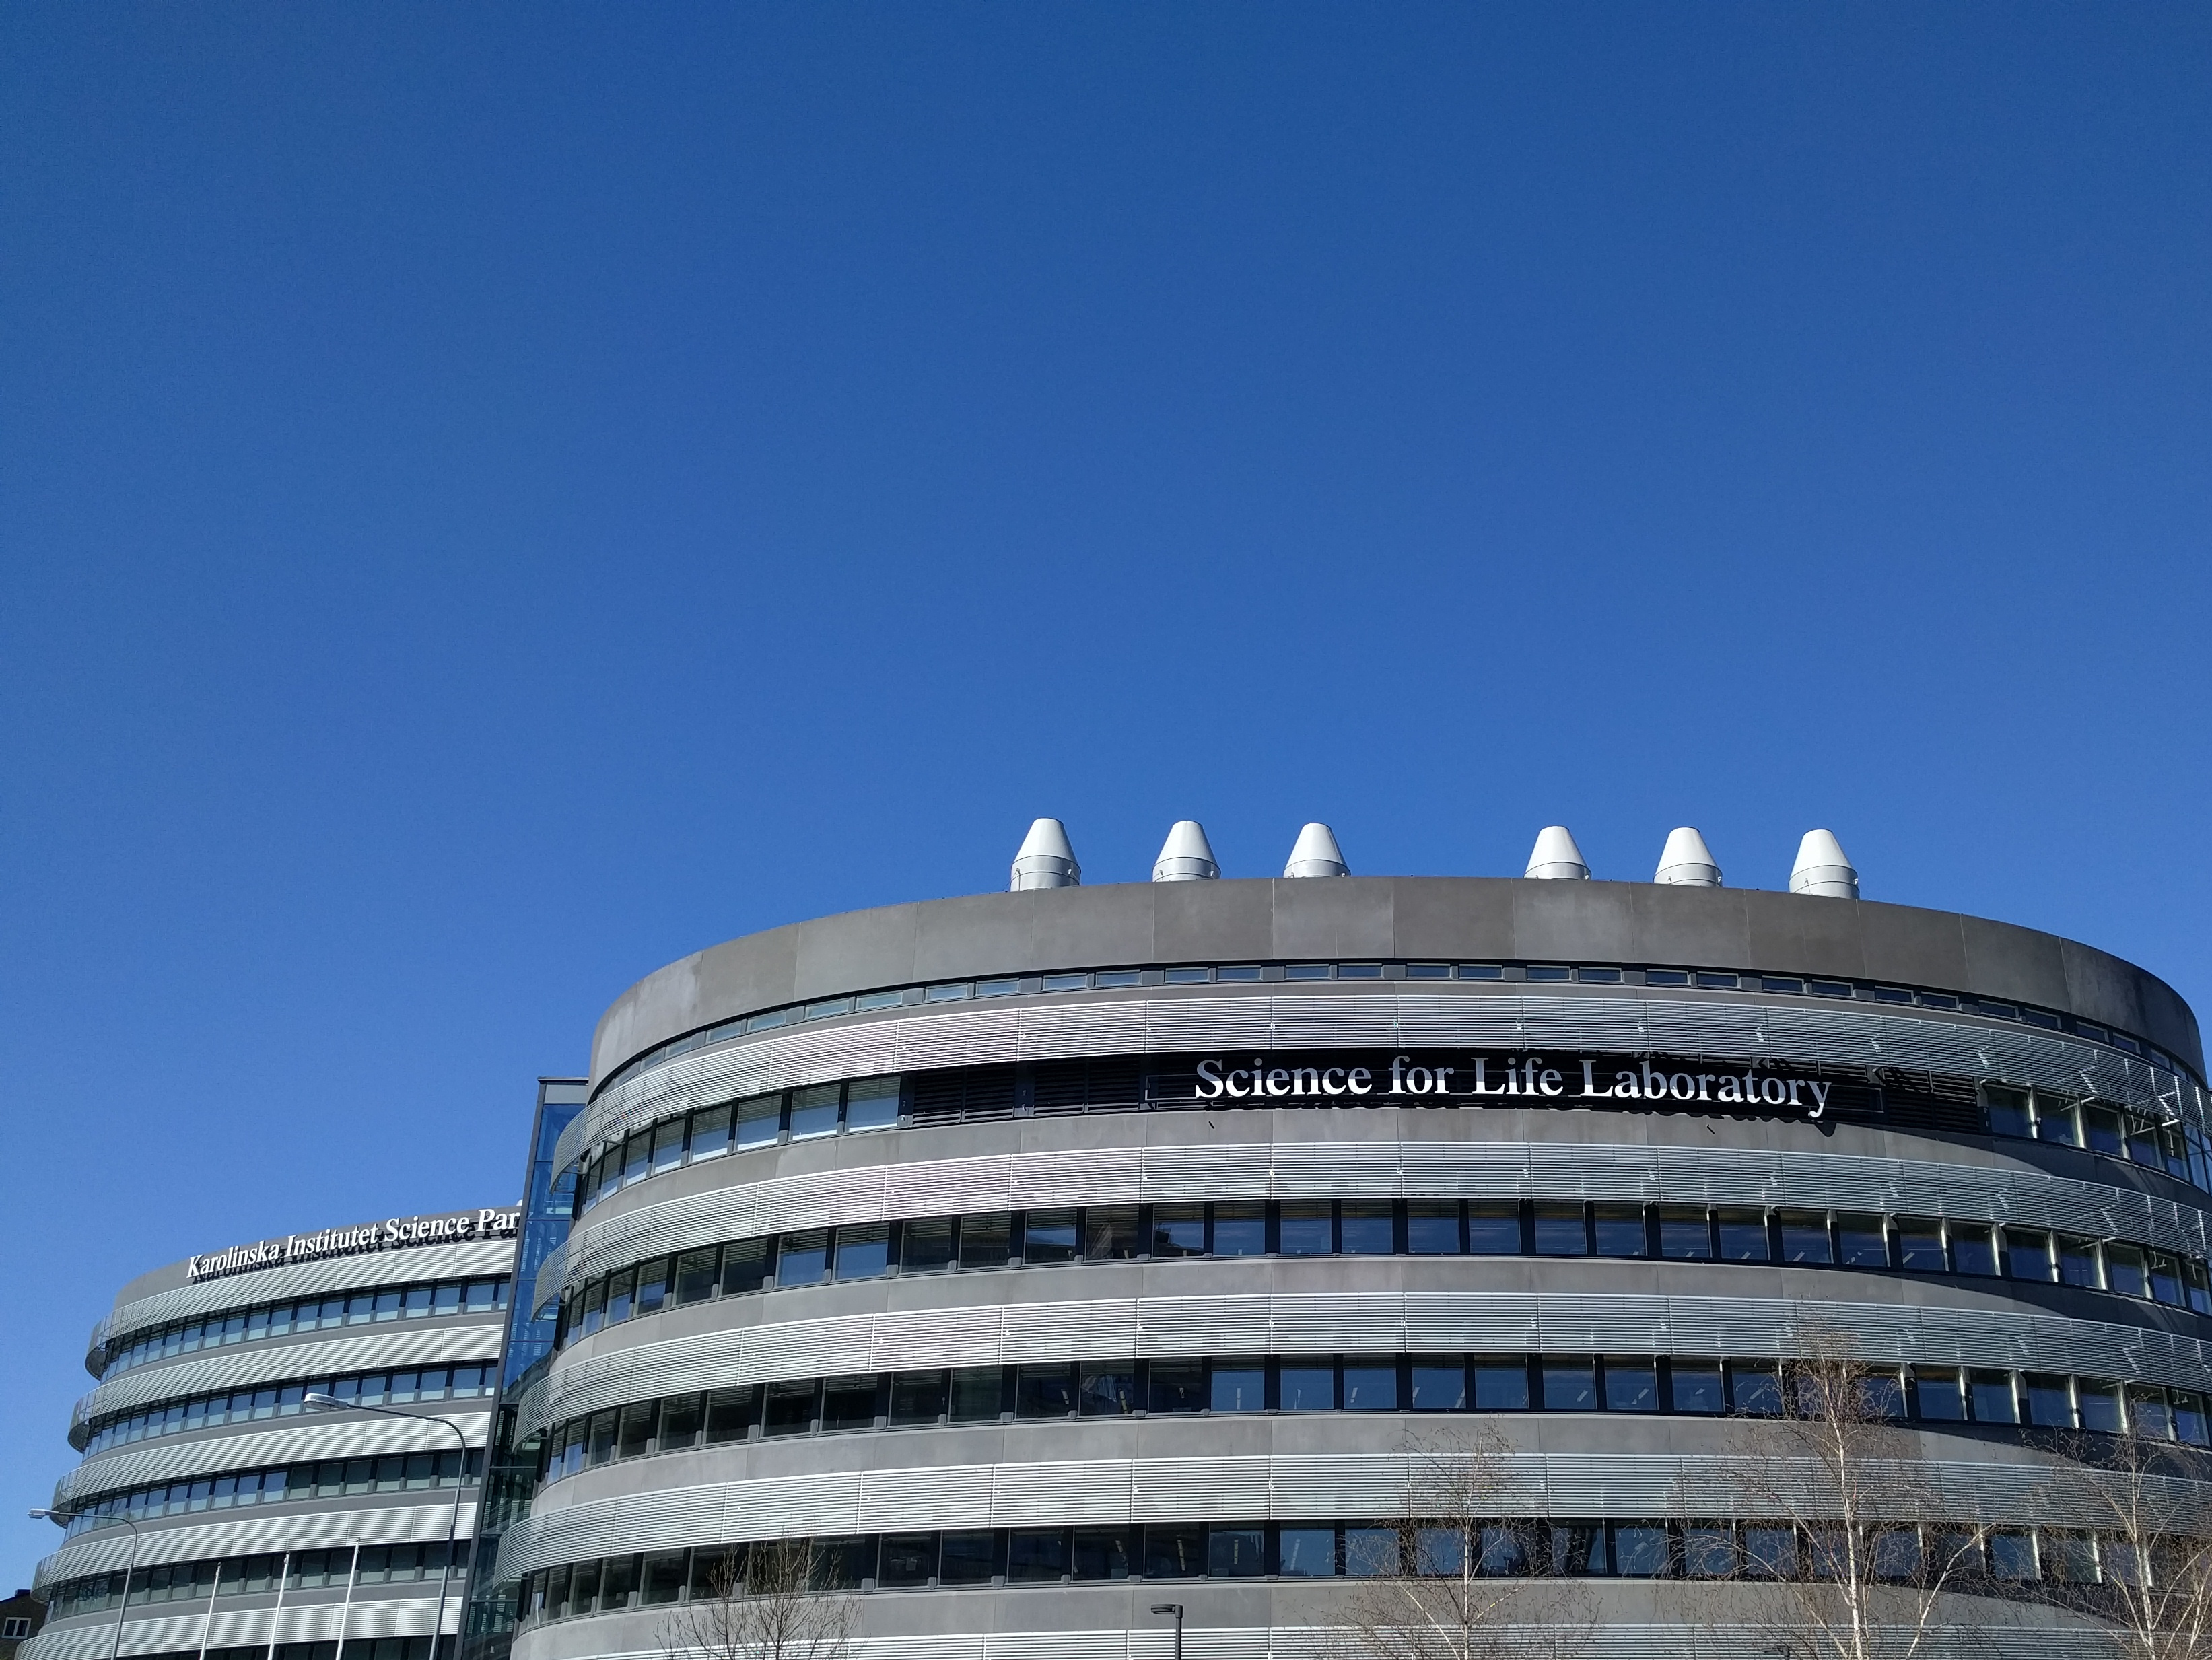
\includegraphics[width=\paperwidth]{pictures/SciLifelab-BlueSky2.jpg}}
	\setbeamercolor{normal text}{fg = white, bg = white}
	\maketitle
}

\section{Sarek}

\begin{frame}{What is Sarek?}
	\begin{figure}
		
\includegraphics[height=1.5cm]{pictures/Sarek_no_border}
		\captionof*{figure}{\faGlobe\ \myurl{http://sarek.scilifelab.se/}}
	\end{figure}
	\begin{itemize}
		\item Analysis germline and somatic workflow
		\item<2-> Whole genome or targeted sequencing
		\item<3-> Developed with NGI and NBIS
		\item<4-> Support from The Swedish Childhood Tumor Biobank
	\end{itemize}
	\begin{figure}
		
\includegraphics[height=.8cm]{pictures/blank}<-2>
		
\includegraphics[height=.8cm]{pictures/NGI}<3->
		\only<4->{\hfill}
		\includegraphics[height=.8cm]{pictures/Barntumörbanken}<4->
		\only<3->{\hfill}
		
\includegraphics[height=.8cm]{pictures/NBIS-orange}<3->
	\end{figure}
	\vfill
\end{frame}

\section{What's inside}

\begin{frame}{Using}
	\begin{figure}
		
\includegraphics[height=1cm]{pictures/nextflow.png}
		\captionof*{figure}{\faGlobe\ \myurl{https://www.nextflow.io/}}
		\only<1>{\captionof*{figure}{ }}
		\only<2>{\captionof*{figure}{Data-driven workflow language}}
	\end{figure}
	\vfill
	\begin{figure}
		
\includegraphics[height=1.5cm]{pictures/Singularity}
		\captionof*{figure}{\faGlobe\ \myurl{https://www.sylabs.io/singularity/}}
		\only<1>{\captionof*{figure}{ }}
		\only<2>{\captionof*{figure}{HPC specific container engine}}
	\end{figure}
\end{frame}

\begin{frame}{Sarek exists in multiple flavors}
	\begin{figure}
		
\includegraphics[height=1.5cm]{pictures/Sarek}
	\end{figure}
	\vfill
	\pause
	\begin{center}
		
\includegraphics[height=1.5cm]{pictures/Sarek_germline}
		\hfill
		
\includegraphics[height=1.5cm]{pictures/Sarek_somatic}
	\end{center}
	\pause
	\begin{figure}
		
\includegraphics[height=1.5cm]{pictures/Sarek_exome}
	\end{figure}
\end{frame}

\begin{frame}{Data and files workflow}
	\begin{figure}
		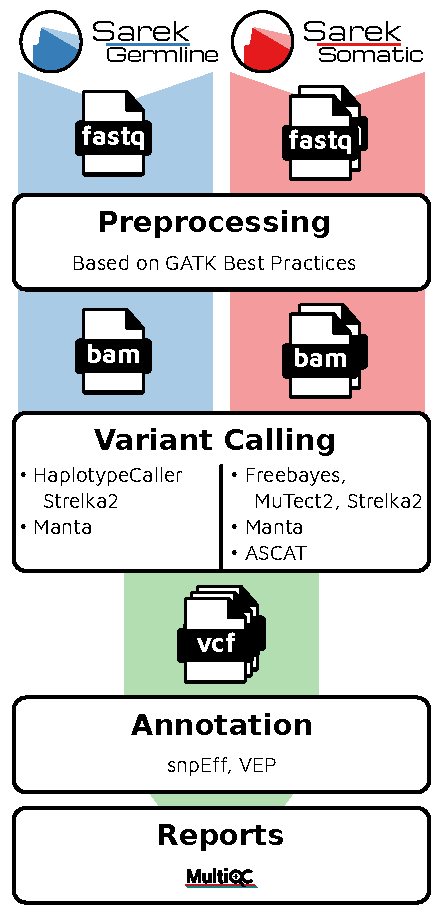
\includegraphics[height=7cm]{pictures/Sarek_2-2_workflow}
	\end{figure}
\end{frame}

\begin{frame}{References Genomes}
	\begin{figure}
		\Huge AWS iGenomes
		\captionof*{figure}{\faGlobe\ \myurl{https://ewels.github.io/AWS-iGenomes/}}
	\end{figure}
	\begin{itemize}
		\item Human \mintinline{text}{GRCh37}
		\item Human \mintinline{text}{GRCh38}
		\pause
		\item Dog \mintinline{text}{CanFam3.1} \faWrench
		\item Mouse \mintinline{text}{GRCm38} \faWrench
	\end{itemize}
\end{frame}

\begin{frame}{Preprocessing}
	\begin{figure}
		
\includegraphics[height=2cm]{pictures/GATKBP}
		\captionof*{figure}{\faGlobe\ \myurl{https://software.broadinstitute.org/gatk/best-practices/}}
	\end{figure}
	Based on GATK Best Practices (GATK 4.0)
	\pause

	\begin{itemize}
		\item Reads mapped to reference genome with \mintinline{text}{bwa mem}
		\pause
		\begin{itemize}
			\item FASTQs or BAMs \faWrench
		\end{itemize}
		\pause
		\item Duplicates marked with \mintinline{text}{picard MarkDuplicates}
		\pause
		\item Recalibrate with \mintinline{text}{GATK BaseRecalibrator}
	\end{itemize}

\end{frame}

\begin{frame}{Variant Calling}
	\begin{itemize}
		\item SNVs and small indels:
		\pause
	\begin{itemize}
			\item Freebayes 
\includegraphics[height=.35cm]{pictures/Sarek_somatic-logo}
			\item HaplotypeCaller 
\includegraphics[height=.35cm]{pictures/Sarek_germline-logo}
			\item MuTect2  
\includegraphics[height=.35cm]{pictures/Sarek_somatic-logo}
			\item Strelka2  
\includegraphics[height=.35cm]{pictures/Sarek_germline-logo}/
\includegraphics[height=.35cm]{pictures/Sarek_somatic-logo}
		\end{itemize}
		\pause
		\item Structural variants:
		\pause
		\begin{itemize}
			\item Manta 
\includegraphics[height=.35cm]{pictures/Sarek_germline-logo}/
\includegraphics[height=.35cm]{pictures/Sarek_somatic-logo}
		\end{itemize}
		\item Sample heterogeneity, ploidy and CNVs:
		\pause
		\begin{itemize}
			\item ASCAT  
\includegraphics[height=.35cm]{pictures/Sarek_somatic-logo}
			\item Control-FREEC \faWrench\  
\includegraphics[height=.35cm]{pictures/Sarek_somatic-logo}
		\end{itemize}
	\end{itemize}
\end{frame}

\begin{frame}{Annotation}
	\begin{itemize}
		\item VEP and SnpEff
		\item \faDatabase\ ClinVar, COSMIC, dbSNP, GENCODE, gnomAD, polyphen, sift, etc.
		\pause
		\item Possibility to use cache directories \faWrench\
		\pause
		\item Prioritization \faWrench\
		\begin{itemize}
			\item Rank scores are computed for all variants, and can be explored
		\end{itemize}
	\end{itemize}
\end{frame}

\begin{frame}{Singularity containers}
	\begin{figure}
		
\includegraphics[height=1.5cm]{pictures/Singularity}
		\captionof*{figure}{\faGlobe\ \myurl{https://www.sylabs.io/singularity/}}
	\end{figure}
	\pause
	\begin{itemize}
		\item Available on \mintinline{text}{rackham} and/or \mintinline{text}{bianca}
		\item \mintinline{text}{/sw/data/uppnex/ToolBox/sarek}
		\pause
		\begin{itemize}
			\item Updated by myself at each new Sarek release
		\end{itemize}
		\pause
		\item Next step \mintinline{text}{Sarek} module
	\end{itemize}
\end{frame}

\begin{frame}{Conda \faWrench}
	\begin{figure}
		
\includegraphics[height=1cm]{pictures/bioconda}
		\captionof*{figure}{\faGlobe\ \myurl{https://bioconda.github.io/}}
	\end{figure}
	\pause
	\begin{itemize}
		\item Execute Sarek within a conda environment
	\end{itemize}
\end{frame}

\begin{frame}{AWS \faWrench}
	\begin{figure}
		
\includegraphics[height=1.5cm]{pictures/AWS}
		\captionof*{figure}{\faGlobe\ \myurl{https://aws.amazon.com/}}
	\end{figure}
	\pause
	\begin{itemize}
		\item Improving AWS usage
	\end{itemize}
\end{frame}

\section{Acknowledgments}

\begin{frame}{Acknowledgments}
	\begin{figure}
		
\includegraphics[height=.6cm]{pictures/Barncancerfonden}%
		\hfill%
		
\includegraphics[height=.6cm]{pictures/KI-horizontal}%
		\hfill%
		\includegraphics[height=.6cm]{pictures/Barntumörbanken}%
		\hfill%
		
\includegraphics[height=.6cm]{pictures/SciLifeLab}%
	\end{figure}
	\begin{table}
		\resizebox{\textwidth}{!}{%
		\begin{tabular}{llllll}
		\textbf{Barntumörbanken}	&	Elisa Basmaci								&	\textbf{NGI}	&	Johannes Alneberg						&	\textbf{NBIS}	&	Sebastian DiLorenzo	\\
															&	Szilveszter Juhos						&								&	Anandashankar Anil					&								&	Malin Larsson	\\
															&	Gustaf Ljungman							&								&	Franziska Bonath						&								&	Marcel Martin	\\
															&	Monica Nistèr								&								&	Orlando Contreras‐López			&								&	Markus Mayrhofer	\\
															&	Gabriela Prochazka					&								&	Phil Ewels									&								&	Björn Nystedt	\\
															&	Johanna Sandgren						&								&	Sofia Haglund								&								&	Markus Ringnér	\\
															&	Teresita Díaz De Ståhl			&								&	Max Käller									&								&	Pall I Olason	\\
															&	Katarzyna Zielinska-Chomej	&								&	Anna Konrad									&								&	Jonas Söderberg	\\
															&															&								&	Pär Lundin									&								&	\\
		\textbf{Grupp Nistèr}	&	Saad Alqahtani			&														&	Remi-Andre Olsen						&	\textbf{Clinical Genomics}	&	Kenny Billiau\\
													&	Min Guo							&														&	Senthilkumar Panneerselvam	&															&	Hassan Foroughi Asl\\
													&	Daniel Hägerstrand	&														&	Fanny Taborsak							&															&	Valtteri Wirta\\
													&	Anna Hedrén					&														&	Chuan Wang									&															&	\\
													&	Martin Proks				&									&							&	\textbf{Nextflow folks}	&	Paolo Di Tommaso	\\
													&	Rong Yu							&									&							&													&	Sven Fillinger	\\
													&	Jian Zhao						&	\textbf{Clinical Genetics}		&	Jesper Eisfeldt			&		&	Alexander Peltzer	\\
		\end{tabular}}
	\end{table}
	\begin{figure}
		
\includegraphics[height=.5cm]{pictures/NGI}%
		\hfill%
		
\includegraphics[height=.5cm]{pictures/NBIS-orange}%
		\hfill%
		
\includegraphics[height=.5cm]{pictures/nextflow.png}%
		\hfill%
		
\includegraphics[height=.5cm]{pictures/nf-core}%
		\hfill%
		
\includegraphics[height=.5cm]{pictures/uppmax.png}%
	\end{figure}
\end{frame}

{
	\usebackgroundtemplate{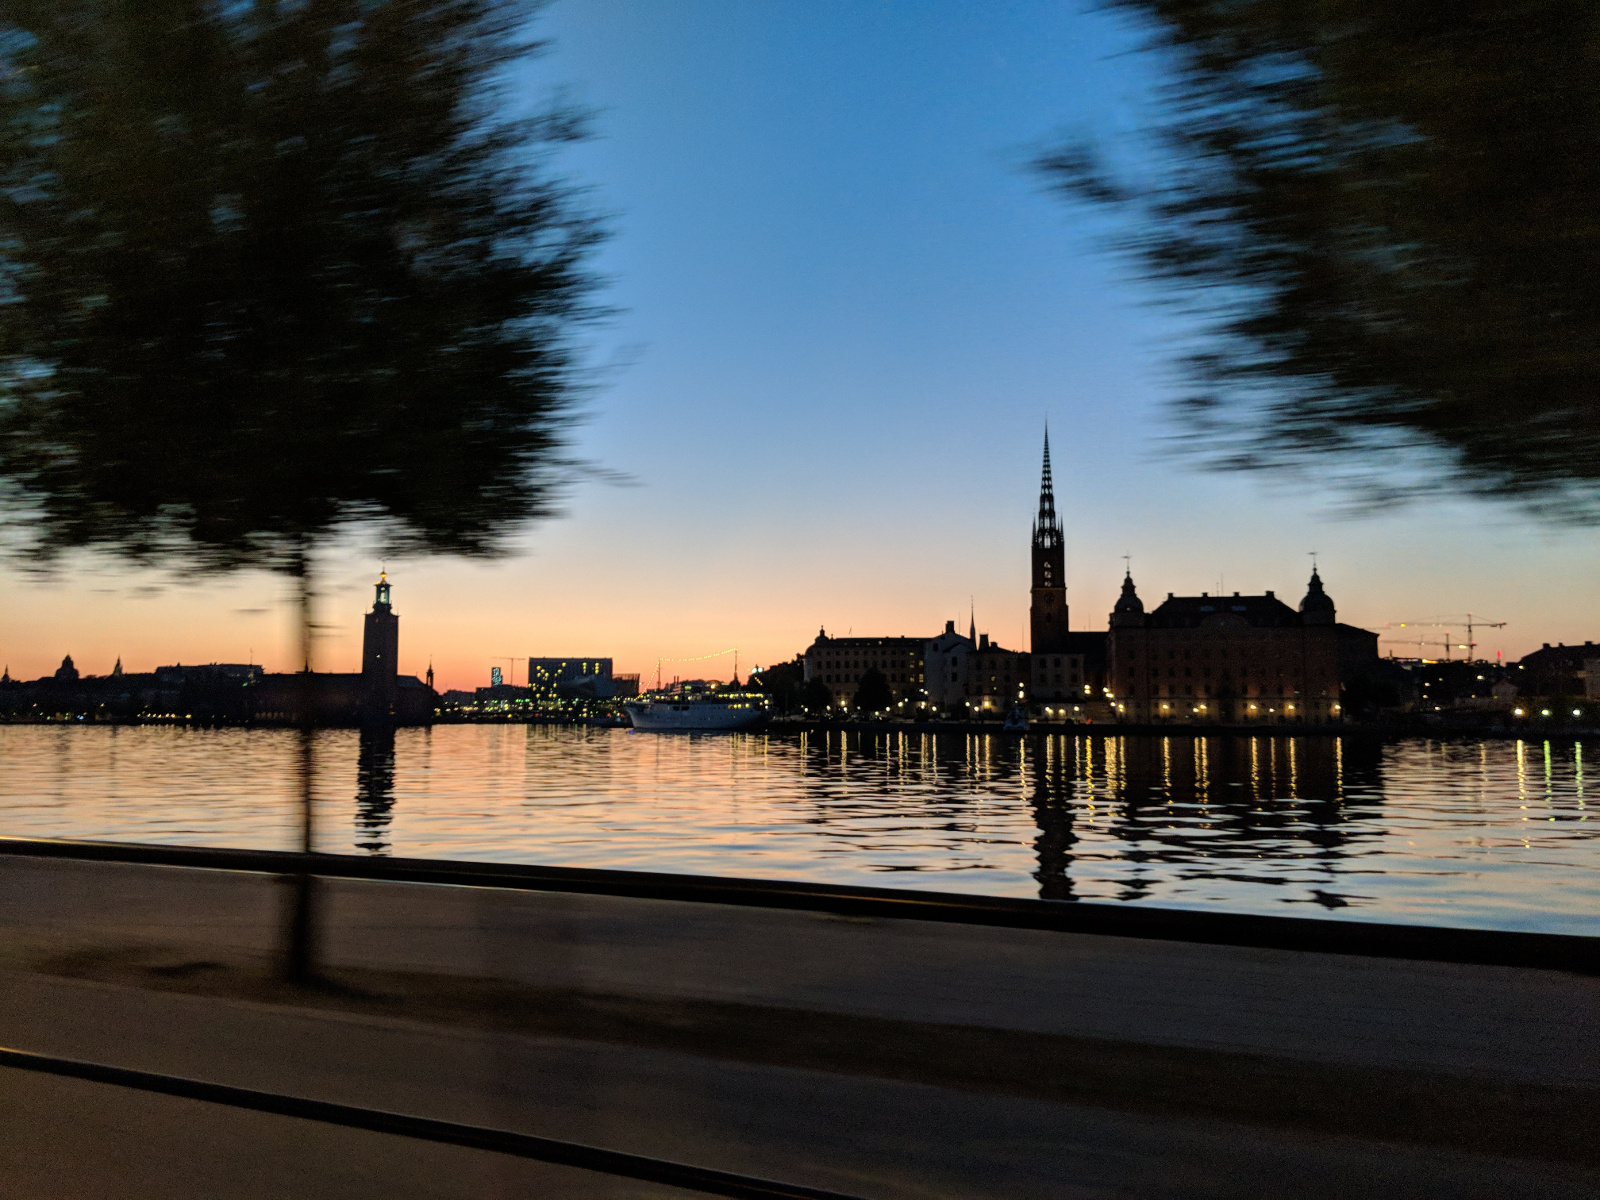
\includegraphics[height=\paperheight]{pictures/Stockholm-by-night.jpg}}
	\setbeamercolor{normal text}{fg = white}
	\setbeamercolor{frametitle}{fg = white, bg = black!80}
	\usebeamercolor[fg]{normal text}
	\section{Questions}
	\begin{frame}[plain]{Any questions?}
		\vspace{-5.3cm}
		\begin{itemize}
			\item[\faGlobe] \url{https://maxulysse.github.io/dnaclub2019}
			\item[\faGithub] \url{https://github.com/SciLifeLab/Sarek}
			\item[\faGitter] \url{https://gitter.im/SciLifeLab/Sarek}
			\item[\faGlobe] \url{http://sarek.scilifelab.se/}
			\item[\faSlack] \#sarek-pipeline
		\end{itemize}
	\end{frame}
}

\end{document}
